\begin{frame}
	\frametitle{Nivel de observaci\'on}
	
	\begin{columns}[T] % contents are top vertically aligned
		\begin{column}[T]{5cm} % each column can also be its own environment
			\begin{itemize}
				\item Captura de datos
				\item Se crean
				\begin{itemize}
					\item Propiedades
					\item Observaciones
				\end{itemize}
			\end{itemize}
		\end{column}
		\begin{column}[T]{5cm} % alternative top-align that's better for graphics
			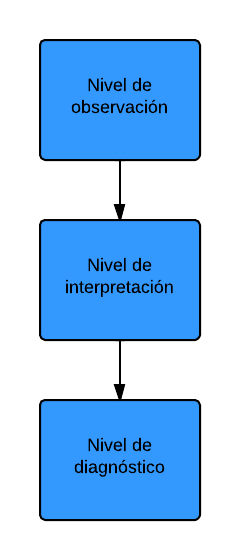
\includegraphics[height=1.0\linewidth]{../Figures/Proceso.png}
		\end{column}
	\end{columns}
\end{frame}